\documentclass[margin=0.5mm]{standalone}
\usepackage{pgfplots}
\usetikzlibrary{pgfplots.groupplots}
\pgfplotsset{compat=1.7}


\begin{document}
	\thispagestyle{empty}

%	\begin{figure}[t]
%		\centering
		
		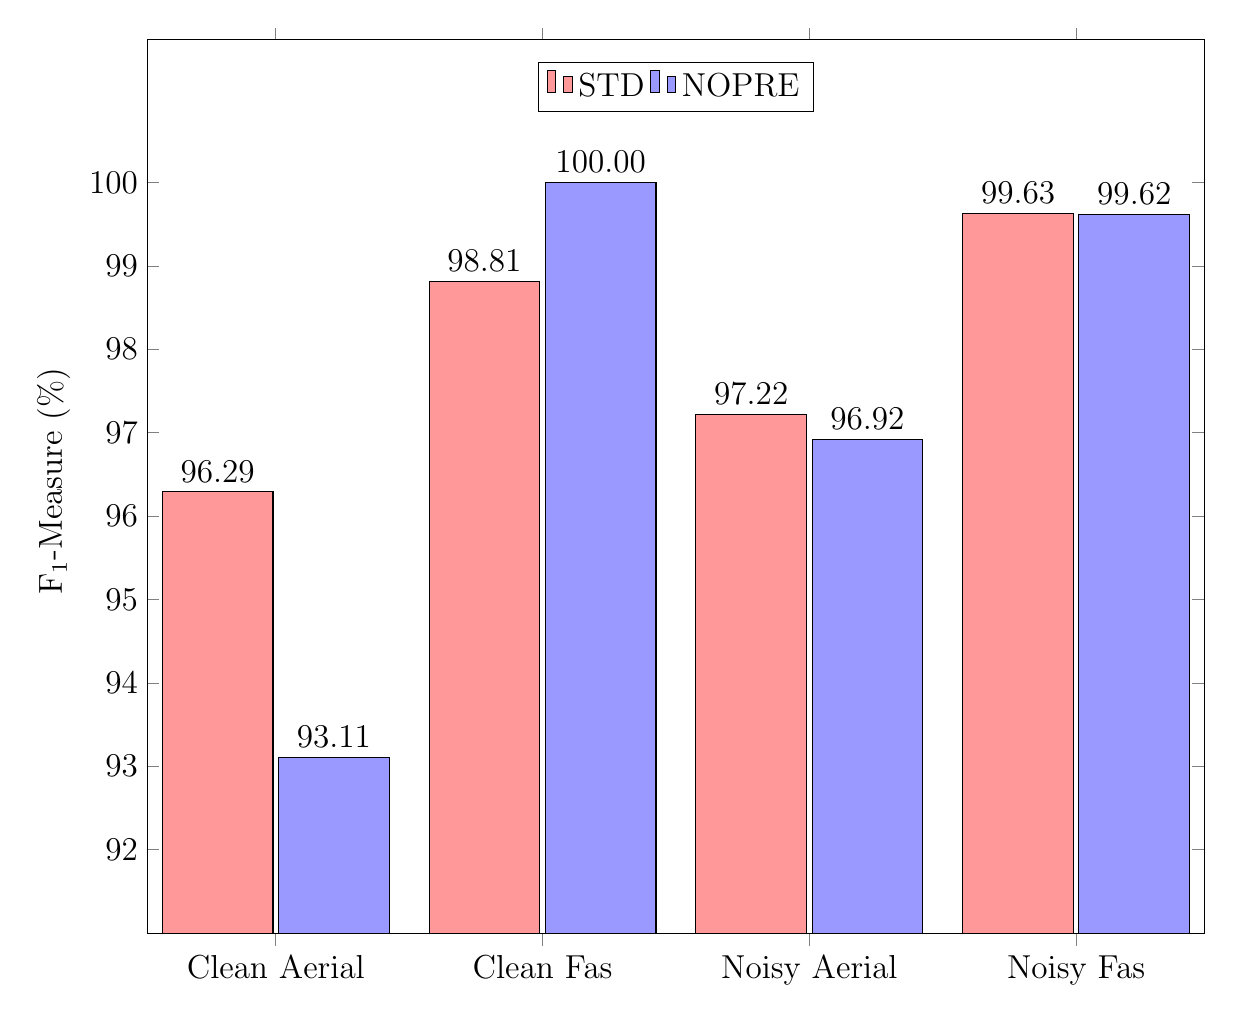
\begin{tikzpicture}
		\begin{axis}[
		width=15cm,
		enlarge x limits=0.16,
		enlarge y limits=0.3,
		ybar,
		%enlargelimits=0.80,
		legend style={at={(0.5,0.975)},
		anchor=north,legend columns=-1},
		ylabel={\ F$_1$-Measure (\%)},
		symbolic x coords={Clean Aerial,Clean Fas,Noisy Aerial,Noisy Fas},
		xtick=data,
		nodes near coords={\pgfmathprintnumber[fixed zerofill, precision=2]{\pgfplotspointmeta}},
		nodes near coords align={vertical},
		bar width=40pt,
		style={font=\large},
		ytick={92,93,...,100},
		ymax=99.7,
		ymin=93
		]
%						STD		NPRE
%			Aerial
%				Clean	96.29	93.11
%				Noisy   97.22   96.92

%			FAS		
%				Clean	98.81	100
%				Noisy   99.625	99.62


		\addplot [color=black,fill=red!40!white] coordinates {(Clean Aerial,96.29) (Clean Fas,98.81) (Noisy Aerial,97.22) (Noisy Fas,99.625) };
		\addplot [color=black,fill=blue!40!white] coordinates {(Clean Aerial,93.11) (Clean Fas,100) (Noisy Aerial,96.92) (Noisy Fas,99.62)};		

		
		\legend{STD,NOPRE}
		\end{axis}
		\end{tikzpicture}
		%\vspace{-0.7cm}
		%\caption{Left: the pitch distribution for the 10 male speakers. Right: the active speech level for the 20 speakers.}\label{fig:pitch}
		%\vspace{-0.5cm}
%	\end{figure}


\end{document}